\section{Степенные ряды}

\begin{Def}
	Функциональный ряд вида $\sum^{+\infty}_{n=0} C_n(x-\alpha)^n = C_0 + C_1(x-\alpha) + ... + C_n(x-\alpha)^n + ...$ называется степенным рядом, $\alpha$ - центр ряда, $C_0, C_1, ...$ - коэффициенты ряда.\\
\end{Def}

\begin{Note}
	$t = x - \alpha \Rightarrow \sum^{+\infty}_{n=0} C_n(x-\alpha)^n = \sum^{+\infty}_{n=0} C_nt^n$ - переместили центр в $0$\\
\end{Note}

\begin{Th}[1-я Теорема Абеля]
	Пусть степенной ряд $\sum^{+\infty}_{n=0} C_n(x-\alpha)^n$ сходится при $x = x_0 \neq \alpha$\\
	Тогда $\forall n, |x-\alpha| < |x_0 - \alpha|$ данный ряд сходится, причём абсолютно, в точке $x$\\
\end{Th}

\begin{Proof}
	$\sum^{+\infty}_{n=0} C_n(x-\alpha)^n$ сходится $\Rightarrow \exists lim C_n(x_0 - \alpha)^n = 0$ (необходимый признак сходимости)\\
	$\Rightarrow C_n(x_0 - \alpha)^n$ ограничена $\Rightarrow \exists M > 0 : \forall n \geq 0 |C_n(x_0 - \alpha)^n| \leq M \Rightarrow |C_n||(x_0 - \alpha)| \leq M$\\
	Возьмём $x : |x-\alpha| < |x_0 - \alpha|$ и пусть $q = \frac{|x - \alpha|}{x_0 - \alpha} \Rightarrow 0 \leq q < 1$\\
	Тогда $\forall n \geq 0 |C_n(x-\alpha)^n| = |C_n||x-\alpha|^n = |C_n||x_0 - \alpha|^nq^n \leq Mq^n$\\
	Ряд $\sum^{+\infty}_{n=0} Mq^n = \frac{1}{1-q}$ сходится, следовательно ряд $\sum^{+\infty}_{n=0} C_n(x-\alpha)^n$ сходится абсолютно по признаку сравнимости\\ 
\end{Proof}

\begin{Note}[Следствие]
	Пусть ряд $\sum^{+\infty}_{n=0} C_n(x-\alpha)^n$ расходится при $x_1 \neq a$, тогда $\forall x |x - \alpha| > |x_1 - \alpha|$ ряд расходится
\end{Note}

\begin{Proof}
	От противного:\\
	Если в условиях следствия $\exists x_0 : |x_0 - \alpha| > |x_1 - \alpha|$ и ряд $\sum^{+\infty}_{n=0} C_n(x_0-\alpha)^n$ сходится, то по теореме ряд $\sum^{+\infty}_{n=0} C_n(x_1-\alpha)^n$ сходится абсолютно, что противоречит условию.\\
	ч.т.д\\
\end{Proof}

\begin{Note}~\\
	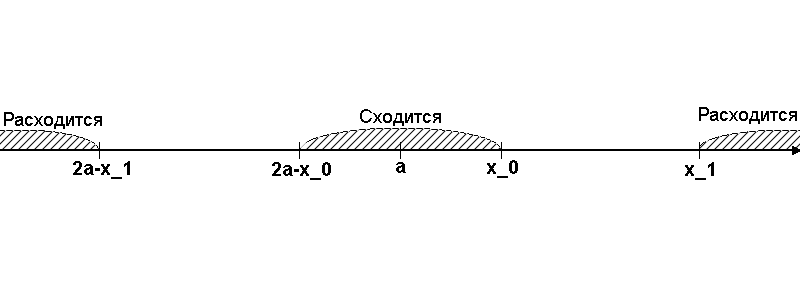
\includegraphics[width = 1\textwidth]{pictures/4_3_1.png}
\end{Note}

\begin{Th}[О существовании радиуса сходимости степенного ряда]
	Пусть $\sum^{+\infty}_{n=0} C_n(x-a)^n$ - степенной ряд\\
	Тогда $\exists R, o \leq R \leq +\infty$, для которого:\\
	1) $\forall x |x-a| < R$ ряд сходится в $x$\\
	2) $\forall x |x-a| > R$ ряд расходится в $x$\\ 
	При этом $R$ - радиус сходимости,  а $(a-R;a+R)$ - интервал сходимости.
\end{Th}

\begin{Proof}
	Если ряд сходится только в $a$, $R = 0$\\
	Если ряд сходится при $\forall x$, $R = +\infty$\\
	Рассмотрим третий случай\\
	$\exists x_0 \neq a$ и ряд сходится в $x_0$\\
	$\exists x_1 \neq a$ и ряд расходится в $x_1$\\
	Для упрощения доказательства перейдём к ряду с центром 0: $\sum\limits_{n=0}^{+\infty}c_nx_n$\\
	Не умаляя общности можно считать, что $x_1 > 0$. Пусть  $E = \{\alpha > 0 | \sum\limits_{n=0}^{+\infty}c_nx_n - \text{расходится}\}$\\
	$R = \inf E \geq x_0 > 0 \Rightarrow R > 0$. Тогда нужно доказать, что: $\begin{cases}
		x > R \Rightarrow$ ряд расходится$\\
		|x| < R \Rightarrow$ ряд сходится$\\
	\end{cases}$
	\begin{enumerate}
		\item $\forall x : \quad 0 \leq |x| < R$ - ряд сходится
		\item $\forall \varepsilon > 0\,\exists x_{\varepsilon} \quad R < x_{\varepsilon} < R + \varepsilon$ ряд расходится в $x_{\varepsilon}$\
		Возьмём $x > R. \quad \varepsilon = x - R > 0 \Rightarrow \exists x_{\varepsilon} \in E \quad R < x_{\varepsilon} < x \Rightarrow [\text{по теореме 2}] \Rightarrow$ ряд расходится в $x$.
	\end{enumerate}
	Итого: 
	$\begin{cases}
	\forall x < R - \text{ряд сходится}\\
	\forall x > R - \text{ряд расходится}
	\end{cases} \Rightarrow$ доказано для $x > 0$. Аналогично доказывается, для $x < 0 \Rightarrow R$ - радиус сходимости ряда
\end{Proof}

\begin{Note}(вычисление радиуса сходимости ряда)\\
	Пусть ряд $\sum\limits_{n=0}^{+\infty}c_n(x-a)^n$
	\begin{enumerate}
		\item $\exists \lim\limits_{n \to +\infty}|\frac{c_{n+1}}{c_n}| = Q \Rightarrow R = \frac{1}{Q} \quad (Q = 0 \Rightarrow R = +\infty; Q = \infty \Rightarrow R = 0)$
		\item $\exists \lim\limits_{n \to +\infty}\sqrt[n]{c_n} = L \Rightarrow R = \frac{1}{L} \quad (L = 0 \Rightarrow R = +\infty; L = \infty \Rightarrow R = 0)$
	\end{enumerate}
\end{Note}

\begin{Proof}
	\begin{enumerate}
		\item Рассмотрим ряд: $\sum\limits_{n=0}^{+\infty}|c_n||x-a|^n$\\
		$a_n = |c_n||x-a|^n \geq 0 (x \neq a, c_n > 0) \Rightarrow\\
		\Rightarrow \frac{a_{n+1}}{a_n} = \frac{|c_{n+1}||x-a|^{n+1}}{|c_n||x-a|^n} = |x-a| \cdot |\frac{c_{n+1}}{c_n}| \rightarrow |x-a| \cdot Q = q$\\
		По признаку Даламбера:$
		\begin{cases}
		q < 1 \Rightarrow $ ряд сходится $\Leftrightarrow |x-a| \cdot Q < 1 \Leftrightarrow |x-a| < \frac{1}{Q}\\$
		$q > 1 \Rightarrow$ ряд расходится $\Leftrightarrow |x-a| \cdot Q > 1 \Leftrightarrow |x-a| > \frac{1}{Q}
		\end{cases}$
		\item $\sqrt[n]{a_n} = |x-a| \sqrt[n]{|c_n|} \rightarrow |x-a| \cdot L = l$\\
		По признаку Коши:$
		\begin{cases}
		l < 1 \Rightarrow $ ряд сходится $\Leftrightarrow |x-a| \cdot L < 1 \Leftrightarrow |x-a| < \frac{1}{L}\\$
		$l > 1 \Rightarrow$ ряд расходится $\Leftrightarrow |x-a| \cdot L > 1 \Leftrightarrow |x-a| > \frac{1}{L}
		\end{cases}$
	\end{enumerate}
\end{Proof}

\begin{Example}~\\
	\begin{enumerate}
		\item $\sum\limits_{n = 0}^{+\infty}\frac{x^n}{n} \quad \quad \frac{c_{n+1}}{c_n} \rightarrow 1 \Rightarrow R = 1 \Rightarrow (-1;1)$ - интервал сходимости
		\item $\sum\limits_{n = 0}^{+\infty}\frac{x^n}{n!} \quad \quad \frac{c_{n+1}}{c_n} = \frac{1}{n} \rightarrow 0 \Rightarrow R = +\infty \Rightarrow$ сходится $\forall x \in \bb{R}$
		\item $\sum\limits_{n = 0}^{+\infty}n! \cdot x^n \quad \frac{c_{n+1}}{c_n} \rightarrow +\infty \Rightarrow R = 0 \Rightarrow$ сходится тлько при $x = 0$
	\end{enumerate}
\end{Example}

\begin{Th}(Вторая теорема Абеля)
	Пусть $R > 0$ - радиус сходимости степенного ряда $\sum\limits_{n=0}^{+\infty}c_n(x-a)^n$.\\
	Тогда $\forall [\alpha; \beta] \subset (a-R; a+R)$ ряд $\sum\limits_{n=0}^{+\infty}c_n(x-a)^n$ сходится равномерно на $[\alpha; \beta]$
\end{Th}

\begin{Proof}~\\
	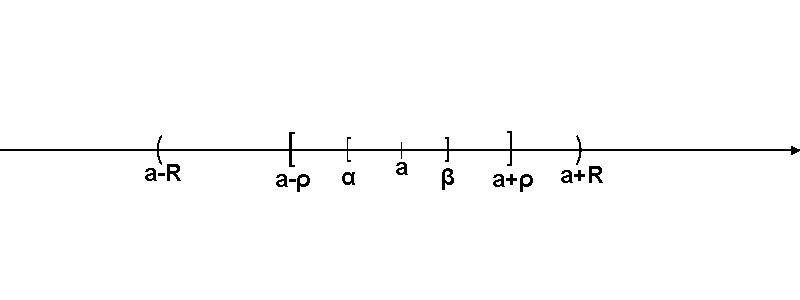
\includegraphics[width = 1\textwidth]{pictures/4_3_2.png}\\
	$\exists \rho < R: [\alpha;\beta] \subset [a-\rho;a+\rho]$, т.е. $a-\rho \leq \alpha < \beta \leq a+\rho, \rho \geq \max {|a-\alpha|;|a-\beta|}$\\
	$\forall x \in [\alpha;\beta] \quad |c_n(x-a)^n| = |c_n||x-a|^n < |c_n| \cdot \rho^n$\\
	$\sum\limits_{n=0}^{+\infty}c_n(x-a)^n$	-- сходится равномерно на $[\alpha;\beta]\\$
	*Сложность была в том, чтобы сделать отрезок сходимости симметричным относительно центра ряда*
\end{Proof}

\begin{Seq}~\\
	Пусть $S(x) = \sum\limits_{n=0}^{+\infty}c_n(x-a)^n, x \in (a-R;a+R), R > 0$.\\
	Тогда $S(x) \in C_{(a-R;a+R)}$
\end{Seq}

\begin{Proof}
	$c_n(x-a)^n \in C_{(a-R;a+R)}$, возьмём $x_0 \in (a-R;a+R), x_0 \in (\alpha;\beta)$, при этом $[\alpha;\beta] \subset (a-R;a+R) \Rightarrow$ ряд сходится равномерно для $[\alpha;\beta] \Rightarrow S(x) \in C_{[\alpha;\beta]} \Rightarrow S(x)$ непрерывна в $x_0$
\end{Proof}

\begin{Seq}~\\
	Пусть $S(x)  = \sum\limits_{n=0}^{+\infty}c_n(x-a)^n, R > 0, x \in (a-R;a+R)$.\\
	Тогда $\forall [\alpha;\beta] \subset (a-R;a+R) \int\limits_{\alpha}^{\beta}S(x)dx = \sum\limits_{n=0}^{+\infty}c_n \cdot \frac{(\beta - a)^{n+1} - (\alpha - a)^{n+1}}{n+1}$, т.к. ряд сходится равномерно на $[\alpha;\beta]$\\
	Если $\alpha = a; \beta = t: \int\limits_{a}^{t}S(x)dx = \sum\limits_{n=0}^{+\infty}\frac{c_n}{n+1}(t-a)^{n+1}, |t-a| < R$ 
\end{Seq}

\begin{Th}(О почленном дифференциировании степенного ряда)
	Пусть $S(x) = \sum\limits_{n=0}^{+\infty}c_n(x-a)^n, R > 0, x \in (a-R;a+R)$.\\
	Тогда
	\begin{enumerate}
		\item $S(x) \in C_{(a-R;a+R)}^{1}$
		\item $S'(x) = \sum\limits_{n=0}^{+\infty}c_n'((x-a)^n)' = \sum\limits_{m=0}^{+\infty}(m+1)c_{m+1}(x-a)^m, x \in (a-R;a+R)$\\
		Причём радиус сходимости этого ряда $R' = R$
	\end{enumerate}
\end{Th}

\begin{Proof}От противного: предположим, что $R' < R$\\
	Для простоты положим $a = 0$. Возьмём $x_0 \in (R';R)$ и $R' < x_0 < x_1 < R, q = \frac{x_1}{x_0} > 1$\\
	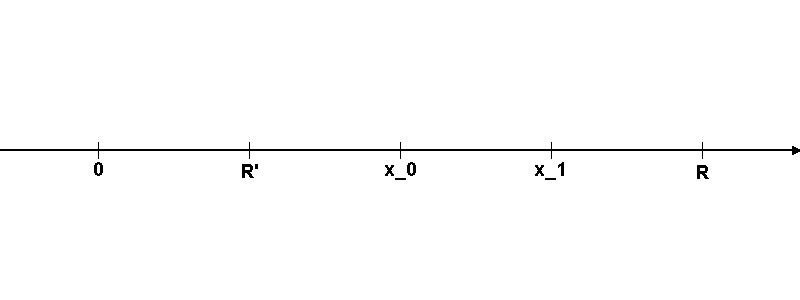
\includegraphics[width = 1\textwidth]{pictures/4_3_3.png}\\
	$\sum\limits_{n=0}^{+\infty}c_nx_0^n$ абсолютно сходится, т.к. $0 < x_0 < R$\\
	$|(n+1)c_{n+1}x_1^n| = (n+1)|c_{n+1}||x_1|^n \leq \frac{(n+1)|c_{n+1}|}{q^n}\cdot x_1^n$\\
	$\lim\limits_{n \to +\infty}\frac{n+1}{q^n} = [\text{По правилу Лопиталя для } lim \frac{+\infty}{+\infty}] = \lim\limits_{t \to +\infty}\frac{1}{q^t\ln(q)} = 0 \Rightarrow \exists n_0 \in \bb{N} \forall n \geq n_0 0 < \frac{n+1}{q^n} < 1 \Rightarrow \forall n \geq n_0 \quad |(n+1)c_{n+1}x_0^n| < |c_{n+1}|x_1^n$\\
	Ряд $\sum\limits_{n = 0}^{+\infty}|c_{n+1}| x_1^{n}$ - сходится при $0 < x_1 < R \Rightarrow \sum\limits_{n=0}^{+\infty}(n+1)c_{n+1}x_0^n$ - абсолютно сходится по признаку сравнения. Но $x_0 > R' \Rightarrow$ ряд расходится. Противоречие $\Rightarrow R' = R$\\
	$S'(x) \in C_{(a-R;a+R)} \Rightarrow S(x) \in C_{(a-R;a+R)}^{1}$
\end{Proof}

\begin{Seq}
	Пусть $S(x) = \sum\limits_{n=0}^{+\infty}c_n(x-a)^n, R > 0, x \in (a-R;a+R)$.\\
	Тогда $\forall k \geq 1 \in \bb{N} \quad S(x) \in C_{(a-R;a+R)}^{k}, S^{(k)}(x) = \sum\limits_{n=0}^{+\infty} \frac{(n+k)!}{n!}\cdot c_{n+k}(x-a)^n, x \in (a-R;a+R)$, т.е. 
	$S(x) \in C_{(a-R;a+R)}^{+\infty}$ - бесконечно дифференциируема
\end{Seq}

\begin{Example}~\\
	$|x| < 1$\\
	$\frac{1}{1-x} = \sum\limits_{n = 0}^{+\infty}x^n \Rightarrow \frac{1}{(1-x)^{k+1}} = \sum\limits_{n=0}^{+\infty}\frac{(n+k)!}{n!k!}\cdot x^n = \sum\limits_{n=0}^{+\infty}c_{n+k}^{k}x^n$
\end{Example}

\begin{Th}(Третья теорема Абеля)
	Пустья числовой ряд $\sum\limits_{n=0}^{+\infty}c_n = S$ сходится, $S \in \bb{R}$\\
	Рассмотрим степенной ряд $S(x) = \sum\limits_{n=0}^{+\infty}c_n x^n, |x| < 1$, т.е. $x \in (-1;1)$\\
	Тогда $\exists \lim\limits_{x \to 1-0}S(x) = S$, т.е. $S(x)$ непрерывна слева в $x = 1$
\end{Th}

\begin{Example}~\\
	\begin{enumerate}
		\item $\frac{1}{1-x} = \sum\limits_{n = 0}^{+\infty}x^n \Rightarrow \frac{1}{1+x} = \sum\limits_{n = 0}^{+\infty}(-1)^nx^n$\\
		$\ln(x+1) = \int\limits_{0}^{x}\frac{dt}{1+t} = \sum\limits_{n=0}^{+\infty}\frac{(-1)^nx^{n+1}}{n+1} = \sum\limits_{n=1}^{+\infty}\frac{(-1)^{n-1} x^n}{n}$\\
		$S = \sum\limits_{n=0}^{+\infty}\frac{(-1)^n}{n}$ - сходится $\Rightarrow$ [по теореме 5] $\Rightarrow S = \lim\lim\limits_{x \to 1 - 0}\ln(1+x) = \ln 2$
		\item $\frac{1}{1+x^2} = \sum\limits_{n = 0}^{+\infty}(-1)^n x^{2n}, |x| < 1$\\
		$\arctan(x) = \int\limits_{0}^{x}\frac{dt}{1+t^2} = \sum\limits_{n=0}^{+\infty}\frac{(-1)^n x^{2n+1}}{2n+1}, |x| < 1 \Rightarrow \sum\limits_{n=0}^{+\infty}\frac{(-1)^n}{2n+1} = [\text{по теореме 5}] = \frac{\pi}{4} \Rightarrow \frac{\pi}{4} = \sum\limits_{n=0}^{+\infty}\frac{(-1)^n}{2n+1}$
	\end{enumerate}
\end{Example}